\chapter{基本理论}\label{prob-stat-base}

\section{概率论}
\subsection{概率计算}
\begin{empheq}{align*}
\Prob(X|Y) &=\frac{\Prob(X,Y)}{\Prob(Y)}=\frac{\Prob(XY)}{\Prob(Z)}=\frac{\Prob(X\cap Y)}{\Prob(Z)}\mtag{条件概率公式}\\
 &=\frac{\Prob(Y|X)\Prob(X)}{\Prob(Y)} \mtag{贝叶斯公式} \\
\Prob(Y)&=\sum_n\Prob(Y, X_n)=\sum_n\Prob(Y|X_n)\Prob(X_n)\mtag{全概率公式}\\
\E(X)&=\E_Y(\E_X(X|Y))\mtag{全期望公式}\\
\E(X|Z)&=\E_Y(\E_X(X|Y)|Z)\\ 
\Prob(X,Y,Z)&=\Prob(X|Y,Z)\Prob(Y|Z)\Prob(Z)\\
p(y|x)&=\int p(y|z)p(z|x)\dif z\\
	f_X(x) &=\int_{-\infty}^{\infty } f(x,y)\dif y=\frac{\partial F(x,y)}{\partial x} \\
f_{X|Y}(x|y)&=\frac{f(x,y)}{f_Y(y)} 
\end{empheq}
\begin{note}
\begin{enumerate}
\item 条件概率的分子有多种不同的写法.但是注意,$P(X,Y)$是简写,完整的写法是$P(X=x,Z=z)$.
\end{enumerate}
\end{note}
\subsection{随机变量}
\subsubsection{密度、分布函数与矩}
求解密度函数的基本思路有:\circled{1}通过CDF求:先求CDF,再求PDF.\circled{2} 归一化:利用正比关系,直接得到密度函数的大致表达示,再进行归一化,得到密度函数.

\begin{empheq}{align}
	\E(X)&=\int_{-\infty}^{\infty} xf(x)\dif x =\int_{-\infty}^{\infty} \dif x \int_{-\infty}^{\infty} xf(x,y)\dif y\\
	\E(\alpha X)&=\alpha \E(X)\\
	\Var(X)&=\E(X-\E X)^2=\E(X^2)-\E^2(X)=\int_{-\infty}^{\infty} (x-E(X))^2f(x)\dif x \\
	\Var(\alpha X)&=\alpha^2 \Var(X)\\
	\Var(X|Y)&=\E(X^2|Y)-\E^2(X|Y) \\
	\E(XY)&=\int_{-\infty}^{\infty}\int_{-\infty}^{\infty} xyf(x,y)\dif x \dif y \\
	\MGF(X)&=\phi(t)=\E(e^{tX})\mtag{矩母函数} \\
	\MGF(X+Y) &=\MGF(X)\cdot\MGF(Y)=\phi_X(t)\phi_Y(t) \\
	\CF(X)&=f(t)=\E(e^{i t X})\mtag{(一元分布)特征函数}\label{prob-characteristic-function} \\
		\CF(X)&=f(\bm{t})=\E(e^{i X^T\bm{t}})\mtag{(多元分布)特征函数} \\
	\E(X^k)&=\frac{1}{i^k}f^{(k)}(0) \\
	p(x) & =\frac{1}{2\pi}\int_{-\infty}^{\infty} e^{-itx}f(t)\dif t\\
\end{empheq}

\begin{note}
	\begin{enumerate}
		\item 分布函数定义为右连续。
		\item 矩母函数对应于$e^{tX}$的级数展开.特征函数相当于$f(x)$的级数展开.
		\item 特征函数一定存在,但矩母函数不一定存在.
	\item 涉及多个随机变量的和时,通常需要多项式定理.对于低阶的,给出一个例子:
	$$(X_1+\cdots+X_N)^4$$
	
	可以分解为:
	\begin{enumerate}
		\item 只有一个变量$X_i^4$:$n$种.
		\item 只有二个变量$X_i^2X_j^2, X_iX_j^3$:从$n$个中任选2个有$\binom{n}{2}$种可能,前者排列有$\frac{4!}{2!2!}=6$种,后者有$\frac{4!}{3!}\times 2=4$(这里乘上2是因为可以是$X_i^3X_j$),共有$14\binom{n}{2}$种.
		\item 有三个变量$X_i^2X_jX_k$:选3个有$\binom{n}{3}$种,排列有$\frac{4!}{2!}\times 3=36$种.
		\item 有四个变量$X_iX_jX_kX_l$:有$\binom{n}{4}\times 4!$种.
	\end{enumerate}
	
	合起来有$n^4$种.根据这个可以计算独立同分布变量和的矩:
	\begin{empheq}{align*}
		\E\left(\sum_{k=1}^nX_k-\sum_{k=1}^n\E X_k\right)^4&=n\E Y^4+6\times \binom{n}{2}\E (Y_i^2Y_j^2)\\
		&=n\E (X-\E X)^4+ 3n(n-1)(\Var X)^2\\
	\end{empheq}
	
	式中$Y_i=X_i-\E X_i$,展开式中含有$Y_i$奇数项的消去,因为$\E(X-\E X)=0$.
\item 给定任意一个一维序列$x_n$,对低阶矩量与$\max,\min$进行估计:
\begin{enumerate}
	\item $\min\leq \mu\leq \max$,这是显然的。
	\item 给定$\mu,\sigma^2$,能否估计$\min,\max$,显然,$\max$不能任意大,$\min$不能任意小。
	
	我们有
\[	\begin{cases}
	\frac{1}{n}\sum X_i=\mu\\
	\inv{n}\sum (X_i-\mu)^2=\sigma^2
	\end{cases}\]

取isotopic变换:$Y_i=\frac{X_i-\mu}{\sigma}$,于是$\mu_Y=0,\sigma^2_Y=1$。那么
\[\begin{cases}
\sum Y_i=0\\
\sum Y_i^2=n
\end{cases}\]
注意第一个方程描述的是$n-1$维超平面,而第二个方程描述的是$n-1$维球面$S^{n-1}$,于是$Y$位于超平面与球面的交界上,而$\min$和$\max$就是最大与最小的坐标分量。注意这里的最大与最小,有两种可能的含义。第一种是指,对于任意一个点,取它的最大与最小的分量。第二种是,对所有的点,它们中最大的和最小的坐标分量,这种不要求最大与最小出现在一个点上。这里考虑第二种。

首先考虑最大的分量,如果只考虑第二个方程,那么取$Y_k^2$最大为$n$,其它的$Y_i$为0。但这样就不满足第一个方程,于是可行的方案是取一个$Y_j^2=Y_k^2=\frac{n}{2}$,然后取$Y_j=-Y_k$,其它为0,刚好满足第一个方程。那么有没有可能$Y_j^2>\frac{n}{2}$呢?假如确实存在这种$Y_j$,那么$\sum_{-j} Y_i^2<\frac{n}{2}$,同时要求$\sqrt{\frac{n}{2}}+\sum_{-g} Y_i=0$,于是$\sum_{-j} Y_i=\sqrt{\frac{n}{2}}$。在平方和的要求下,其项之和能否达到$\sqrt{\frac{n}{2}}$呢?

可以使用Jensen不等式\eqref{jensen's-in-eq},即$E(f(X))\geq f(E(X))$,$f$是凸函数。取$f=x^2$。那么$\frac{n}{2}\inv{n-1}>\inv{n-1}\sum_{-j} Y_i^2\geq \left(\inv{n-1}\sum_{-j}Y_i\right)^2$,于是$\sum_{-j}Y_i<\sqrt{\frac{n(n-1)}{2}}$,当$n>2$时,上界$\sqrt{\frac{n(n-1)}{2}}>\sqrt{\frac{n}{2}}$则$\sum_{-j} Y_i=\sqrt{\frac{n}{2}}$还是有可能达到的。所以这样考虑不行。

另一种思路是考虑能否直接算出方程的解。比如圆与直线交于两点,而球面与平面交于一个圆。首先由和为0,有$y_{n}=-\sum_{k=1}^{n-1}y_k$,于是
$$\sum_{k=1}^{n-1}y_k^2+\left(-\sum_{k=1}^{n-1}y_k\right)^2=n$$

上式可以改写为
\begin{empheq}{equation}
\begin{bmatrix}
y_1&\cdots&y_{n-1}
\end{bmatrix}\begin{bmatrix}
2& 1 &\cdots &1\\
1& 2 & \cdots &1\\
& & \cdots & \\
1& 1 & \cdots &2
\end{bmatrix}\begin{bmatrix}
y_1\\\cdots\\y_{n-1}
\end{bmatrix}=n
\end{empheq}
取$\bm{y}^T=\begin{bmatrix}
	y_1&\cdots&y_{n-1}
\end{bmatrix}$,则上式是在说
$$\bm{y}^TA_{n-1}\bm{y}=\bm{y}^T(I_{n-1}+\bm{1}_{(n-1)\times(n-1)})\bm{y}=n$$

矩阵$A_n$是对称正定矩阵,其特征值为$\begin{bmatrix}
n& 1& 1&\cdots& 1
\end{bmatrix}$,即恰有一个特征值为$n$,其它全为1。取Cholesky分解$A_{n-1}=L_{n-1}L_{n-1}^T$,则$(L_{n-1}^T\bm{y})^TL_{n-1}^T\bm{y}=n$,又取$L_{n-1}^T\bm{y}=\bm{u},\bm{y}=(L_{n-1}^T)^{-1}\bm{u}$,显然$u_i$的最大可能值是$\sqrt{n}$。那么我们现在希望通过$\bm{u}$的最大值来反算$y_i$的最大值。

由于$A_{n-1}$的特殊结构,可以算出来
$$(L_{n-1}^T)^{-1}=\begin{bmatrix}
\frac{\sqrt{2}}{2} & -\frac{\sqrt{6}}{6}&\cdots &\cdots\\
0& \frac{\sqrt{6}}{3}& -\frac{\sqrt{3}}{6}&\cdots&\cdots\\
& & \cdots& & \\
& & & & \frac{\sqrt{n(n-1)}}{n}\\
\end{bmatrix}$$
这个矩阵的特征是最后一个元素的绝对值是最大的,而主对角线上元素是递增的。要使$y_i$尽可能大,那么应该让$u_{n-1}=\sqrt{n}$,即最后一个元素取最大,前面全为0(这里似乎不太严格,但结论应该是正确的)。于是$y_{\max}=\sqrt{n}\frac{\sqrt{n(n-1)}}{n}=\sqrt{n-1}$,其它元素全为$-\frac{1}{\sqrt{n-1}}$。很容易验证序列和为0,而平方和为$n$。正是我们所需要的。

最终我们有结论
$$\max\leq \mu+\sqrt{n-1}\sigma,\ \min\geq -(\mu+\sqrt{n-1}\sigma)$$
\end{enumerate}

\item 对正值随机变量,可以按如下方式计算期望:
\begin{empheq}{equation}
\E(X)=\int_{0}^{\infty}1-F(x)\dif x
\end{empheq}
这是因为
\begin{empheq}{align*}
\int_{0}^{\infty} xf(x)\dif x&=\left. xF(x)\right\vert_{0}^{\infty} -\int_{0}^{\infty} F(x)\dif x\\
&=\int_{0}^{\infty}1-F(x)\dif x
\end{empheq}
\end{enumerate}
\end{note}
\begin{empheq}{align*}
F^{-1}(p)&=q_p=\inf\{x:F(x)\geq p\}\mtag{$p$分位数}\\
&=\argmin_c \E\left(\rho_p(X-c)\right)\\
\rho_p(x)&=\left(p-I(x<0)\right)x 
\end{empheq}

分位数的性质可以用于进行分位数估计.注意期望与中位数不是同一回事.

\subsubsection{随机变量的和、差、积、商}
\begin{empheq}{align*}
\E(aX)&=a\E(X)\\
\E(X+Y)&=\E(x)+\E(Y)\\
\Var(ax)&=a^2\Var(X)\\
\Var(X+Y)&=\Var(X)+\Var(Y)+2\Cov(X,Y)\\
\Cov(X,Y)&=\E(XY)-\E(X)\E(Y)\\
f_{X+Y}(z)&=\int_{-\infty}^{\infty} f_{XY}(x,z-x)\dif x \mtag{卷积}
\end{empheq}

\subsubsection{随机变量的变换}
假设$X$的密度与分布函数分别为$F_X,f_X$,则它的变换$Y=g(X)$的密度函数按以下计算:
\begin{empheq}{align*}
P(Y\leq y)&=P(X\leq g^{-1}(y))\\
&=F_X(g^{-1}(y))
\end{empheq}
求导有$f_Y(y)=f_X(g^{-1}(y))\left|\frac{\dif g^{-1}(y) }{\dif y}\right|=\left|\frac{f_X(g^{-1}(y))}{g'(y)}\right|$。注意不要把$g^{-1}(y)$当成倒数,它是反函数。

以上假定$g$是单调的。

多元分布同样有:
$$f_Y(\by)=f_X(g^{-1}(\bx))\left|\det\sbra{\frac{\dif g^{-1}(\by)}{\dif \by}}\right|$$

\subsubsection{Censored与Truncated分布}
自然界中的分布都是有界的,对于超出界的样本,如果把它调整为上界或者下界,就是Censor,对应Censored分布;如果直接删除,就是Truncate,对应Truncated分布。

给定一个连续分布的分布函数$F(x)$和密度函数$f(x)$,及上下界$[a,b]$,那么Censored分布的密度函数为
\[
f_{\text{censored}}=\begin{cases}
F(a) & \text{ if } x=a\\
f(x) & \text{ if } a<x< b\\
F(b) & \text{ if } x=b\\
0& \text{ otherwise }
\end{cases}
\]

\[
f_{\text{truncated}}=\begin{cases}
\frac{f(x)}{F(b)-F(a)} & \text{ if } b\leq x\leq a\\
0& \text{ otherwise }
\end{cases}
\]

对于truncated分布,其分布函数为:
\begin{empheq}{equation}
F_{\text{truncated}}=\begin{cases}
0&x<a\\
\frac{F(x)-F(a)}{F(b)-F(a)}& a\leq x<b\\
1&\text{否则}
\end{cases}
\end{empheq}

\subsubsection{多元随机变量的分布与密度}
给定随机向量的分布函数$F(W\bx)$,则密度函数为$f_X(W\bx)|W|$.注意后面还有个行列式.

\subsubsection{条件分布}
\begin{empheq}{align}
\E(g(X)|h(X,Y)=v)&=\int_{-\infty}^{\infty} g(x)f(x|h(X,Y)=v)\dif x
\end{empheq}
\begin{example}
已知$X,Y\sim i.i.d. \Exp(\lambda)$,求$\E(X^2|X+Y)$。

\begin{empheq}{align*}
\E(X^2|X+Y)&=\int_{0}^{v}x^2f(x|v)\dif x\\
f(x|v)&=\frac{f(x,v)}{f(v)}=\pdv[order=2]{F(x,v)}{v}\bigg/\pdv{F(v)}{v}\\
F(x,v)&=\int_{0}^{x}\dif x \int_{0}^{v-x}f(x)f(y)\dif y\\
F(v)&=\int_{0}^{v}\dif x \int_{0}^{v-x}f(x)f(y)\dif y\\
f(x,v)&=\lambda^2 e^{-\lambda v}\\
f(v)&=\lambda^2 ve^{-\lambda v}\\
\implies f(x|v)&=\inv{v}\\
\implies \E(X^2|X+Y)&=\inv{3}v^2
\end{empheq}
注意$f(u|v)$是一个均匀分布,这是一个很特殊的情形。
\end{example}
\subsubsection{多元随机变量的矩}
\begin{empheq}{align*}
	\E(A\bx)&=A\E(\bx)\\
	\text{Var}(A\bm{x})&=A\text{Var}(\bm{x})A^T=A\Sigma A^T	\\
	\E(\bm{x}^T\bm{x})&=\text{trace}(\Sigma)+\bm{\mu}^T\bm{\mu}\\
	\E(\bm{x}\bm{x}^T)&=\Sigma+\bm{\mu}\bm{\mu}^T\\
	\E(\bx a^T\bx)&=\E(\bx\bx^T\bm{a})=\E(\bx\bx^T)\bm{a}\\
	\E(\bx^TA\bx)&=\text{trace}(A\Sigma)+\bm{\mu}^TA\bm{\mu}\\
    \E((A\bx+\bm{a})^T(B\bx+\bm{b}))&=\trace(A\Sigma B^T)+(A\bmu+\bm{a})^T(B\bmu+\bm{b})
\end{empheq}


\subsubsection{相关系数与协方差阵}
\paragraph*{协方差阵}是对称、半正定矩阵,要求特征值全大于等于0.

\paragraph*{线性相关系数}最常见:
$$\rho_{XY}=\frac{\E(XY)-\E(X)\E(Y)}{\sqrt{\Var(X)}\sqrt{\Var(Y)}}=\frac{\Cov(X,Y)}{\sigma_X\sigma_Y}$$

可以看出不同的协方差可以诱导相同的相关系数,那么从协方差阵可以导出相关系数矩阵,但从相关系数矩阵,不一定能导出协方差阵,需要配合方差才行.

而且从定义可以看出,相关系数的定义与向量的夹角基本相似,给定三个向量$X,Y,Z$,假如$X,Y$和$Y,Z$的夹角是给定的:$\theta_1,\theta_2$,那么$X,Z$的夹角也有一个范围:$[|\theta_1-\theta_2|,\theta_1+\theta_2]$.

相应地,相关系数也不能随便设定.

\begin{example}
令$\sigma_X=\sigma_Y=\sigma_Z=1,\mu_X=\mu_y=\mu_Z=0$,假如$\rho_XY=0.5,\rho_YZ=0$,分别对应夹角$\frac{\pi}{3},\frac{\pi}{2}$,那么$\rho_{XZ}\leq\cos\left(\frac{\pi}{2}-\frac{\pi}{3}\right)=\cos\left(\frac{\pi}{6}\right)\approx 0.86625$.协方差阵为
$$\begin{bmatrix}
1 & 0.5 & \rho_{XZ}\\
0.5 & 1 & 0\\
\rho_{XZ}&0&1
\end{bmatrix}$$

当$ \rho_{XZ}\geq 0.866025$时,矩阵就不正定了.

\end{example}
\subsubsection{特征函数}
\ref{prob-characteristic-function}给出了特征函数的定义,它实际上相当于随机变量分布函数的傅里叶变换,是概率论研究的基本工具。矩母函数与特征函数相似,只是指数中没有$i$,显然矩母函数不一定存在,因为实数指数函数是无界的,而特征函数一般是存在的。

\paragraph*{证明中心极限定理}

\subsubsection{分布表}
\paragraph*{离散随机变量}离散随机变量一般都有很明确的意义:

\begin{enumerate}
	\item \emph{Bernoulli分布}:做一次实验,问是否成功的分布情况,实际上成功概率是$p$.
	\item \emph{Binomial分布}:做$n$个Bernoulli实验,问成功次数的分布情况.即$Y=\sum X_k$.
	\item \emph{Negative Binomial分布(Pasca分布)}:重复做Bernoulli实验,直到恰好成功$k$次,则实验失败次数的分布.它与Binomial恰好相反,Binomial分布是已知实验次数,问成功次数.而Negative Binomial是已知成功次数.
	
	Negative Binomial是离散分布,推广到连续情形,就是Polya分布.
	\item \emph{Poisson分布}:$\lambda$是单位时间内事件发生的平均次数,Poisson分布描述的是某段时间内事件发生次数的分布.
	
	Poisson分布是由二项分布推导来的,当$n$很大、$p$很小时,二项分布的极限就是Poisson分布.
	
	Poisson分布与指数分布可以对应起来,指数分布描述的是泊松过程中,事件发生的间隔的分布.
	
\end{enumerate}
\paragraph*{连续随机变量}有些连续随机变量有特殊性质:

\begin{enumerate}
	\item \emph{Normal分布}:最著名的连续分布,因为中心极限定理指出,假如若干种随机变量相互独立地发挥作用,那么极限情况下就趋于正态分布.
	
	它的一大特点是概率密度很快衰减到0,但实际中的数据经常出现长尾的情况,此时可以用t分布建模.不过t分布的计算量远比正态分布高.
	\begin{property}
	
	\begin{enumerate}
		\item 正态分布完全由一阶矩与二阶矩决定.
		\item 多个独立正态分布的随机变量之和,仍是正态分布.
		\item 多维正态分布的条件与边缘分布,仍是正态分布.
        \item 若$X\sim \mathcal{N}(\mu, \sigma^2)$,则$Y=\frac{X-\mu}{\sigma}\sim\mathcal{N}(0,1)$,此时$F_Y(y)=\Phi\left(\frac{y-\mu}{\sigma}\right)$,但$f_Y(y)=\inv{\sigma}\phi\left(\frac{y-\mu}{\sigma}\right)$,注意密度函数需要缩放。
	\end{enumerate}
\end{property}
	大致上可以看出,正态分布天然是“线性分布”.
	
	求正态分布方差的简便方法:
	
	\begin{empheq}{align*}
		&\int_{-\infty}^{\infty}\frac{1}{\sqrt{2\pi}\sigma}e^{-\frac{x^2}{2\sigma^2}}\dif x=1\\
		\xRightarrow{\text{对}\sigma\text{求导}}& \int_{-\infty}^{\infty} \frac{1}{\sqrt{2\pi}}\frac{-1}{\sigma^2}e^{-\frac{x^2}{2\sigma^2}}+\frac{1}{\sqrt{2\pi}\sigma}e^{-\frac{x^2}{2\sigma^2}}\frac{-x^2}{2}(-2)\frac{1}{\sigma^3}\dif x=0\\
		\xRightarrow{\text{整理}}&\int_{-\infty}^{\infty}x^2\frac{1}{\sqrt{2\pi}\sigma}e^{-\frac{x^2}{2\sigma^2}}\dif x=\sigma^2
	\end{empheq}
	
	对于多元正态分布,如果想证明积分为1,首先对协方差矩阵进行分解,进行变量替换使协方差阵成为对角矩阵,一下就可以得到积分为1.
	
	\item \emph{t分布}:常用的长尾分布,当自由度很高时,趋近于正态分布.
    
    \begin{property}
    \begin{enumerate}
    \item $1<\nu\leq 2$时,分布的方差无穷大,所以一般在软件中进行回归时,$\nu$一般默认取3。
    \item $k$阶矩只在$0<k<\nu$时有定义,更高阶矩不存在。
    \item 标准化:如果$X\sim t_{\nu}(\mu,\sigma)$,那么$\frac{x-\mu}{\sigma}\sim t_{\nu}$,这里是标准t分布。
    \item 缩放:如果$X\sim t_{\nu}(\mu,\sigma)$,那么$\alpha X+\beta\sim t_{\nu}(\alpha \mu+\beta, \alpha\sigma)$。
    \end{enumerate}
    \end{property}
	\item \emph{Chi-square分布}:标准正态分布的平方和就是卡方分布:$Y=\sum X_i^2,\ X_i\sim N(0,1)$.
	\item \emph{Exponential分布}:无后效性.
	\item \emph{Wishart分布}:描述的是正定对称矩阵的分布,比如协方差阵,或者估计理论中常用的$X^TX$的分布.
	$$\forall \mathbf{x}\in \mathcal{R}^d,\ \cfrac{\mathbf{x}^TS \mathbf{x}}{\mathbf{x}^T W \mathbf{x}}\sim \chi_{\nu-d-1}^2,\text{ given }W\sim \text{Wishart}_{\nu,d}(S),\ \nu>d-1$$
	
	大致可以看出,Wishart分布就是Chi分布的多维推广.
	
	如果取$S=I$,那就是标准Wishart分布.
    \item \emph{Weibull分布}.经常用于可靠性分析。当$k=1$时,它是指数分布,$k=2$时是Rayleigh分布。
	\item \emph{次高斯分布}.简单地说就是比高斯分布衰减得更快的分布:
	$$\exists C,v>0,\ \Prob(|X|>t)\leq Ce^{-vt^2}$$
	
\end{enumerate}

\paragraph*{由随机变量的和差积商导出的分布}这些分布通常用于统计检验,一般假设随机变量间是独立的.
\begin{enumerate}
\item \emph{F分布}
$$\frac{\chi_{d_1}/d_1}{\chi_{d_2}/d_2}\sim F(d_1,d_2)$$
\end{enumerate}
\paragraph*{共轭分布}
\begin{enumerate}
\item 如果$X|\mu\sim N(\mu,\sigma^2),\sigma^2\sim IG(\frac{\nu}{2},\frac{\nu}{2}s^2)$,那么
$$X\sim t_{\nu}\left(\mu, \frac{s^2}{n}\right)$$
\end{enumerate}

\newpage
\thispagestyle{empty}
\newgeometry{left=1.5cm,bottom=0.5cm,top=0.5cm,right=1.5cm}
\begin{landscape}
\begin{longtable}{X{0.15\linewidth} X{0.1\linewidth} X{0.35\linewidth}Y{0.1\linewidth}X{0.2\linewidth}}
\toprule
\heiti{分布}& \heiti{记号} & \heiti{密度函数}  &\hfil \heiti{矩} & \heiti{特征函数}\\
\midrule
\multirow{3}{*}{Binomial}&\multirow{3}{*}{ $X\sim\text{Bin}(n,p)$}&\multirow{3}{*}{ $\binom{n}{k}p^k(1-p)^{n-k}$}& $\E(X)=np$ & \multirow{3}{*}{$\left(1-p+pe^{it}\right)^n$}\\
& & &$\Var(X)=np(1-p)$ & \\
& & & mode$(X)=$& \\
\midrule
\multirow{3}{*}{Negative Binomial}&\multirow{3}{*}{ $X\sim\text{Neg-Bin}(\alpha,\beta)$}&\multirow{3}{*}{ $\binom{\alpha-1+k}{\alpha-1}\left(\frac{\beta}{\beta+1}\right)^\alpha\left(\frac{1}{\beta+1}\right)^\alpha$}& $\E(X)=\frac{\alpha}{\beta}$ & \multirow{3}{*}{$\left(\frac{1-p}{1-pe^{it}}\right)^n$}\\
& & &$\Var(X)=\frac{\alpha}{\beta^2}(\beta+1)$ & \\
& & & mode$(X)=$& \\
\midrule
\multirow{3}{*}{Beta Binomial}&\multirow{3}{*}{ $X\sim\text{Beta-Bin}(n,)$}&\multirow{3}{*}{ $$}& $E(X)=$ & \multirow{3}{*}{$$}\\
& & &$D(X)=$ & \\
& & & mode$(X)=$& \\
\midrule
\multirow{3}{*}{Uniform} & \multirow{3}{*}{$X\sim \text{U}(a,b)$}&\multirow{3}{*}{$\frac{1}{b-a}$} & $\E(X)=\frac{b-a}{2}$&  \\
& & &$\Var(X)=$ & \\
& & & & \\
\midrule
\multirow{3}{*}{Normal}&\multirow{3}{*}{ $X\sim \text{N}(\mu,\sigma^2)$}&\multirow{3}{*}{ $\frac{1}{\sqrt{2\pi}\sigma}e^{-\frac{(x-\mu)^2}{2\sigma^2}}$}& $\E(X)=\mu$& \multirow{3}{*}{$e^{i\mu t-\frac{1}{2}\sigma^2 t^2}$}\\
& & &$\Var(X)=\sigma^2$ & \\
& & & mode$(X)=\mu$& \\
\midrule
\multirow{3}{*}{Lognormal}&\multirow{3}{*}{ $X\sim\text{lognormal}(\mu,\sigma^2)$}&\multirow{3}{*}{ $\frac{1}{\sqrt{2\pi}\sigma x}e^{-\frac{(\ln x-\mu)^2}{2\sigma^2}}$}& $\E(X)=e^{\mu+\frac{1}{2}\sigma^2}$ & \multirow{3}{*}{$$}\\
& & &$\Var(X)=e^{2\mu+\sigma^2}(e^{\sigma^2}-1)$ & \\
& & & mode$(X)=e^{\mu-\sigma^2}$& \\
\midrule
\multirow{3}{*}{Skew Normal}&\multirow{3}{*}{ $X\sim\text{SkewNormal}(\mu,\sigma,\alpha)$}&\multirow{3}{*}{ $\frac{2}{\sigma}\phi(\frac{x-\mu}{\sigma})\Phi\Big(\alpha\Big(\frac{x-\mu}{\sigma} \Big)\Big)$}& $\E(X)=\mu+\sqrt{\frac{2}{\pi}}c\sigma,\ c=\frac{\alpha}{\sqrt{1+\alpha^2}}$ & \multirow{3}{*}{$e^{i\mu t-\frac{\sigma^2}{2}t^2}$}\\
& & &$\Var(X)=\Big(1-\frac{2c^2}{\pi}\Big)\sigma^2$ & \\
& & & mode$(X)=$& \\
\midrule
\multirow{3}{*}{Multivariate Normal}&\multirow{3}{*}{ $X\sim\text{N}_d(\bm{\mu},\Sigma)$}&\multirow{3}{*}{ $(2\pi)^{-\frac{d}{2}}|\Sigma|^{-1/2}e^{-\frac{1}{2}(\bm{x}-\bm{\mu})^T\Sigma^{-1}(\bm{x}-\bm{\mu})}$}& $\E(X)=\bm{x}$ & \multirow{3}{*}{$e^{i\bm{\mu}^T\bm{t}-\frac{1}{2}\bm{t}^T\Sigma \bm{t}}$}\\
& & &$\Var(X)=\Sigma$ & \\
& & & mode$(X)=\bm{\mu}$& \\
\midrule
\multirow{3}{*}{Gamma}&\multirow{3}{*}{ $X\sim\text{Gamma}(\alpha,\beta)$}&\multirow{3}{*}{$\frac{\beta^\alpha}{\Gamma(\alpha)}x^{\alpha-1}e^{-\beta x}$}& $\E(X)=\frac{\alpha}{\beta}$ & \multirow{3}{*}{$\Big(1-\frac{it}{\beta}\Big)^{-\alpha}$}\\
& & &$\Var(X)=\frac{\alpha}{\beta^2}$ & \\
& & & mode$(X)=\frac{\alpha-1}{\beta}$& \\
\midrule
\multirow{3}{*}{t}&\multirow{3}{*}{ $X\sim\text{t}_\nu(\mu,\sigma^2)$}&\multirow{3}{*}{ $\frac{\Gamma(\frac{\nu+1}{2})}{\Gamma(\frac{\nu}{2})\sqrt{\nu \pi}\sigma}\left(1+\frac{1}{\nu}\left(\frac{x-\mu}{\sigma}\right)^2\right)^{-\frac{\nu+1}{2}}$}& $\E(X)=\mu$ & \multirow{3}{*}{$$}\\
& & &$\Var(X)=\frac{\nu}{\nu-2}\sigma^2$ & \\
& & & mode$(X)=\mu$& \\
\midrule
\multirow{3}{*}{Multivariate t}&\multirow{3}{*}{ $X\sim\text{t}_\nu(\bmu,\Sigma)$}&\multirow{3}{*}{ $\frac{\Gamma(\frac{\nu+1}{2})}{\Gamma(\frac{\nu}{2})(\nu\pi)^{d/2}}|\Sigma|^{-\inv{2}}\left(1+\frac{1}{\nu}(\bx-\mu)^T\Sigma^{-1}(\bx-\mu)\right)^{-\frac{\nu+d}{2}}$}& $\E(X)=\bmu$ & \multirow{3}{*}{$$}\\
& & &$\Var(X)=\frac{\nu}{\nu-2}\Sigma$ & \\
& & & mode$(X)=\bmu$& \\
\midrule
\multirow{3}{*}{Wishart}&\multirow{3}{*}{ $X\sim\text{Wishart}_{\nu,d}(S)$}&\multirow{3}{*}{ $\cfrac{|W|^{\frac{\nu-d-1}{2}}e^{-\frac{1}{2}\text{tr}(S^{-1}W)}}{2^{\frac{\nu d}{2}}|S|^{\frac{\nu}{2}}\Gamma_p\left(\frac{d}{2}\right)}$}& $\E(X)=dS$ & \\
& & &$\Var(X)=$ & \\
& & & mode$(X)=$& \\
\midrule
\multirow{3}{*}{Inverse Wishart}&\multirow{3}{*}{ $X\sim\text{Inv-Wishart}_{\nu,d}(S)$}&\multirow{3}{*}{ $\cfrac{|S|^{\frac{\nu}{2}}e^{-\frac{1}{2}\text{tr}(S^{-1}W)}}{2^{\frac{\nu d}{2}}|W|^{\frac{\nu-d-1}{2}}\Gamma_p\left(\frac{d}{2}\right)}$}& $\E(X)=dS$ & \\
& & &$\Var(X)=$ & \\
& & & mode$(X)=$& \\
\midrule
\multirow{3}{*}{Weibull}&\multirow{3}{*}{ $X\sim\text{Weibull}(\lambda,k)$}&\multirow{3}{*}{ $\frac{k}{\lambda}\left(\frac{x}{\lambda}\right)^{k-1}e^{-(x/\lambda)^{k}}$}& $\E(X)=\lambda \Gamma\left(1+\inv{k}\right)$ & \\
& & &$\Var(X)=$ & \\
& & & mode$(X)=$& \\
\midrule
\multirow{3}{*}{Dirichlet}&\multirow{3}{*}{ $X\sim\text{Dirichlet}(\balpha)$}&\multirow{3}{*}{$\frac{\Gamma(\sum \alpha_k)}{\prod \Gamma(\alpha_k)}x_1^{\alpha_1-1}\cdots x_n^{\alpha_n-1},\sum x_k=1$}& $\E(X)=\frac{\alpha_k}{\sum \alpha_k}$ & \multirow{3}{*}{$\Big(1-\frac{it}{\beta}\Big)^{-\alpha}$}\\
& & &$\Var(X)=\frac{\alpha}{\beta^2}$ & \\
& & & mode$(X)=\frac{\alpha-1}{\beta}$& \\
\bottomrule
\end{longtable}
\end{landscape}

\newpage
\restoregeometry

\subsubsection{随机变量的分类}
\begin{description}
\item[isotropic] 期望为$\bm{0}$,协方差为$I$的随机变量(或随机向量)。对于任意随机变量$X$,按$\Sigma^{-1/2}(X-\mu)$变换后的随机变量是isotropic的。
\item[log-concave] 如果随机变量的密度函数$f$满足
$$f(\lambda x+(1-\lambda)y)\geq f(x)^\lambda f(y)^{1-\lambda}$$
则称它为log-concave,均匀分布、指数族分布等等均属于此类,实际上常见的分布函数基本上都是这样的。
\end{description}
\subsection{大数定律、渐近理论、Concentration Inequality与KLS猜想}
三者非常相似,都是考查随机变量在大样本下的分布情况。Concentration描述的现象是,大多数概率分布,其密度函数分布在一个比较小的区间内,可以说是一种“富集”现象。由于这种将就的存在,采样时只需要在一个小的区域内进行,就可以得到相当准确的估计。
\subsubsection{次高斯分布}
\begin{theorem}{Boucheron 2013\cite{Boucheron2013_conineq}}
假如$X$是一个$\sigma^2$-次高斯分布,那么有
$$\Prob(X\geq \epsilon)\leq \exp\sbra{-\frac{\epsilon^2}{2\sigma^2}}$$
\end{theorem}
\subsection{采样方法}
\subsubsection{反函数方法}
适用于一元随机变量。假设目标分布为$F(X)$,首先随机生成$x_i\sim U[0,1]$值,再计算$F^{-1}(x_i)$,所得序列就符合目标分布。

\subsubsection{重要性采样}
\paragraph*{基本方法}
它要解决的问题是估计
$$\E(f(\bx)),\bx\sim p$$
如果我们能直接从$p$中进行采样,则可以直接用
$$\E(f(\bx))\approx \inv{N}\sum f(\bx_k)$$
来估计。如果不能从$p$中采样,但知道密度函数$p$的具体形式,可以考虑用一个$q$来逼近$p$,这是重要性采样的出发点。假设$p(\bx)=\inv{Z}\phi(\bx)$,则
$$Z=\int \phi(\bx)\dif \bx = \int \frac{\phi(\bx)}{q(\bx)}q(\bx)\dif \bx \approxeq \inv{N} \sum w(\bx_i)$$
此外$\bx_i\sim q$。那么
\begin{empheq}{align}
\E(f(\bx))&=\inv{Z}\int f(\bx)\phi(\bx)\dif \bx\\
&=\inv{Z}\int f(\bx)\frac{\phi(\bx)}{q(\bx)}q(\bx)\dif \bx\\
&\approxeq \frac{1}{NZ}\sum f(\bx_i)w(\bx_i)\\
&=\frac{\sum w(\bx_i)f(\bx_i)}{\sum w(\bx_i)}\\
&=\sum W(\bx_i)f(\bx_i)=\hat{\mu}\mtag{重要性采样逼近}
\end{empheq}
显然$q$要足够接近$\phi$或者$p$,重要性采样逼近的效果才会比较好。

逼近的方差为:
\begin{empheq}{align*}
\Var(\hat{\mu})&=\inv{N}\left(\int \frac{f^2(\bx)p^2(\bx)}{(q\bx)}\dif \bx\right)
\end{empheq}
对于一个给定的$N$,假如$f^2(\bx)p^2(\bx)$的衰减速度慢于$q(\bx)$,比如前者是一个长尾分布,则$\Var(\hat{\mu})\rightarrow \infty $。
\subsubsection{随机变量的采样}
\paragraph*{一元正态分布}

\paragraph*{多元正态分布}

\paragraph*{多元t分布}

\paragraph*{Gamma分布}

\subsection{统计检验}
统计检验的基本思想是构造统计、计算它的分布、计算$p$值.

基本统计量如下:
\begin{empheq}{align*}
S^2&=\frac{1}{n-1}\sum_{k=1}^{n}(X_i-\bar{X})\mtag{样本方差}
\end{empheq}

\subsubsection{F检验}
\paragraph*{正态总体检验方差一致}两组数据的样本方差分别为$S_1^2,s_2^2$.
$$\frac{S_1^2}{S_2^2}\sim F(n_1-1,n_2-1)$$
\subsection{Copula}
Copula是一种处理高维分布的工具.

\subsubsection{Copula基础概念}
\begin{definition}{Copula}{}
\begin{empheq}{align*}
F(x_1,x_2,\cdots,x_n)&=C(u_1,u_2,\cdots,u_n) \mtag{Sklar Theorem}\\
&=C(F_1(x_1),F_2(x_2),\cdots,F_n(x_n))\\
f(x_1,x_2,\cdots,x_n)&=c(F_1(x_1),F_2(x_2),\cdots,F_n(x_n))\prod_{k=1}^{n}f_k(x_k)
\end{empheq}

$C$函数被称为Copula.强调单独给定$C$函数时,联合分布仍然是未知的,还需要边缘分布信息.
\end{definition}

Sklar定理将多元随机变量的分布函数,表示为每个随机变量的分布函数的函数.

在二维的情形有:
\begin{empheq}{align*}
f(x_1,x_2)&=\frac{\partial^2 F(x_1,x_2)}{\partial x_1\partial x_2}\\
&=\frac{\partial^2 C_{12}(F_1(x_1),F_2(x_2))}{\partial x_1\partial x_2}\\
&=c_{12}(F_1(x_1),F_2(x_2))f_1(x_1)f_2(x_2)\\
c_{12}(u_1,u_2)&=\frac{\partial^2 C_{12}(u_1,u_2)}{\partial u_1\partial u_2}\\
f(x_2|x_1)&=c_{12}(F_1(x_1),F_2(x_2))f_2(x_2)
\end{empheq}

Vine Copula是高维Copula的一种表示方法,用多棵树表示高维分布.比如对于一个三维Copula,有以下分解:
\begin{empheq}{align*}
f(x_1,x_2,x_3)=&f_1(x_1)f_2(x_2)f_3(x_3)\text{ (marginals)}\\
&\cdot \textcolor{blue}{c_{12}(F_1(x_1),F_2(x_2)) c_{23}(F_2(x_2),F_3(x_3))}\text{ (unconditional) }\\
&\cdot \textcolor{red}{c_{13|2}(F_{1|2}(x_1|x_2),F_{3|2}(x_3|x_2))}\text{ (conditional)}
\end{empheq}

对应于两棵树
\begin{center}
\begin{tikzpicture}[
	basicnode/.style={circle,draw=black, very thick, minimum size=7mm},
	blueline/.style={draw=blue}
	]
	%Nodes
	\node[basicnode]   (N1)   {1};
	\node[basicnode,right=2.5cm of N1]  (N2)    {2};
	\node[basicnode,right=2.5cm of N2]      (N3)  {3};
	%Lines
	\path[blueline] (N1)--node[midway,above,align=center]{\textcolor{blue}{12}} (N2);
	\path[blueline] (N2)--node[midway,above,align=center]{\textcolor{blue}{23}} (N3);
\end{tikzpicture}
\end{center}

\begin{center}
\begin{tikzpicture}[
	basicnode/.style={circle,draw=black, very thick, minimum size=7mm},
	redline/.style={draw=red}
	]
	%Nodes
	\node[basicnode]      (N12)                              {12};
	\node[basicnode,right=3cm of N12]        (N23)  {23};
	%Lines
	\path[redline] (N12)--node[midway,above,align=center]{\textcolor{red}{13|2}} (N23);
\end{tikzpicture}
\end{center}

在第二棵树中,结点12和13都包含2,所以是指“给定2”的情况下,即条件分布.

\subsubsection{常用的Copula}
\begin{longtable}{X{0.1\textwidth} X{0.5\textwidth} X{0.2\textwidth}}
\toprule
名称& 形式 参数范围 \\
\midrule
Gumbel& $e^{-\left((-\ln u_1)^\theta+(-\ln u_2)^\theta\right)^{1/\theta}}$ &$\theta\in[1,\infty)$\\
\bottomrule
\end{longtable}

\subsubsection{理解Copula}
单独给定一个二元Copula函数$C(u_1,u_2)$,其实不能得到边缘分布,它跟边缘分布无关.通常拟合Copula时,要先将原始数据进行积分变换成为$[0,1]$区间内.常见的做法是可以假定一个边缘分布,计算分位数,或者使用经验分布函数进行变换.然后将变换后的数据代入Copula函数进行拟合,在拟合时,其实没有用到边缘分布.

那么使用Copula函数与用一般的二元分布有什么区别呢?

答案在于Copula的范围更广,比如一个连续分布是正态,一个是t分布,可以用Copula来描述相关性.一般的做法是使用二维正态分布或者t分布,显然范围就缩小了.

另一方面,由于Copula没有直接使用边缘分布,所以使用可以完整地保留连续分布的信息.但这并不一定是好事,假如希望得到边缘分布,还得要设定分布形式来估计.

现在再看相关系数,相关系数中需要联合分布,所以不同的Copula下,利用公式计算的相关系数可能不同.比如我们首先对两个变量拟合不同的Copula,再进行模拟生成$u_1,u_2$、还原为原变量,并计算相关系数.预期不同的Copula诱导的相关系数不同.

模拟的一种简便方法是先随机生成$u_1$,再反算$u_2$.

\section{极值理论}
主要考查诸如局部极值、最大与最小值的分布一类的问题。
\subsection{局部极值的分布}

\subsubsection{图上随机函数的局部极值数量分布}
\cite{distribution-of-local-minima-of-graph}指出:
\begin{theorem}{图上随机函数的局部极值数量分布}
给定一个$d$图$G(V,E)$,即每个节点有$d$个相邻节点,又令$F$是一个$G$上的随机函数,且在每个节点处的值是独立分布的(只限定连续,不限定分布的具体类型)。取$W$为$F$的局部极值数量,又取$\E(W)=\mu,\Var (W)=\sigma^2$,则
$$\E (W)=\frac{|V|}{d+1}$$
且对于任意正数$w$,有
$$\left|\Prob(W\leq w)l-\Phi\left(\frac{w-\mu}{\sigma}\right)\right|\leq\frac{C}{\sqrt{\sigma}}$$
\end{theorem}

这个定理是在说,局部极值的分布接近正态分布。但文章作者也认为这个上界不是紧的,最优的界(收敛速度)可能与$\inv{\sigma}$成正比,而不是$\frac{1}{\sqrt{\sigma}}$。

以下给出一些应用的例子:
\begin{enumerate}
	\item 对于一个$n\times n$的二维网格,假设边界是周期性的,则每个点有4个相邻节点,$d=4$,那么$|V_n|=n^2$,
	$$\E(W_n)=\frac{n^2}{5}$$
	
\end{enumerate}
\section{随机过程}
\subsection{随机过程的基本概念}

\subsubsection{什么是随机过程}
\paragraph*{定义}
随机过程就是一个随机变量族$\{X_t\}_{t\in\Omega}$,$\Omega$是下标集合,最常见的就是$\mathbb{N}$,即以时间为下标,但它也可以是实数集或者其它抽象集合。它由有穷维分布函数族完全确定,所谓有空维分布就是取一个有限子集$\{X_t\}_{t\in\omega}$的联合分布。随机过程从本质上来说就是无穷维的,但我们不可能直接定义一个无穷维的分布,所以只能用有限维分布来刻画。

从以上可以看出,理解一个随机过程需要抓住三个要素:
\begin{description}
	\item[下标集$\Omega$] 下标集可以是任意一个无限集,并不必然是整数。
	\item[随机变量的值域$E$] 值域就是每个随机变量的取值。
	\item[有穷维分布] 它刻画了随机过程的概率性质。随机变量是无限维的,只能通过“切片”的方式来刻画,一个切片就是一个联合分布。但在定义一个随机变量时,我们不必给出任意子集的有穷维分布,可以只给出某些特定子集的分布,Dirichlet过程就是一个例子。
	
	对随机过程进行采样,就是对某个有穷维分布进行采样(我们不可能对无限个随机变量的联合分布采样),所以就要首先确定这个有穷维分布对应的下标集。
\end{description}

注意随机过程有多种类型,每种类型定义的出发点不同:
\begin{enumerate}
\item 增量过程,值域可以连续或者离散。增量可以是独立的,比如独立增量过程,也可以有相关性,比如Ito过程属于此类。适合描述动力系统。
\item 直接给定同质有空维分布族。比如高斯过程就是任何子集的随机变量满足高斯分布。高斯过程的下标集是自然数。

Dirichlet过程就是某些特定有空维分布为Dirichlet分布,此时它的下标集是集合的幂集。

并非任何分布都能够作为有空维分布族。高斯过程是因为高斯分布的特性:子集也属于高斯分布。但服从多元t分布的子集不一定满足t分布,所以就没有t过程。
\item 马尔科夫过程。取值离散,下一时刻的状态由之前的状态决定。
\end{enumerate}
从以上可以看出Ito过程只是随机过程的一个子类,不要混淆机器学习中的随机过程与Ito过程。

\paragraph*{实现}定义并不能直接告诉我们应当如何得到随机过程的一个实现(或者说采样)。

\paragraph*{应用}随机过程适合用来描述无穷维的东西:
\begin{enumerate}
\item 以时间或者自然数为下标的变量族,比如时间序列回归或者一般的回归。此时每个样本对应一个随机变量。
\item 描述整数下标本身,每个下标可以对应其它的东西。比如聚类分布中聚类的数量,又比如无限个基函数。注意区别它与上一点,两种情况下,下标都有其对应的东西,但上一点中,我们希望刻画的是下标对应的东西,而这里,我们是希望刻画下标本身,通常是给下标确定一个概率。
\item 划分。比如把一个区间划分为若干份,划分的数量可以趋于无穷。
\end{enumerate}
\subsubsection{Ito微积分}
用于对以随机过程为变量的函数进行微分。

\paragraph*{基本原理}
\begin{empheq}{align*}
\int_{0}^{t}\dif B_s&=\sum_{i=1}^{N}B_{s_{i}}-B_{s_{i-1}}=B_t\\
\dif t\dif t&=\dif t\dif B_t=0\\
\dif B_t\dif B_t&=\dif t\\
\end{empheq}
这里是从随机游走的极限情况考虑的。在$\Delta t$时间的内的增量$\Delta B_t$服从正态分布$N(0,\Delta^2 t)$。

现在考虑积分
\begin{empheq}{align*}
\int_{0}^{t}B_s\dif B_s&=\sum B_{s_i}(B_{s_i}-B_{s_{i-1}})\\
&=\sum\left(-\frac{1}{2}\left((B_{s_i}-B_{s_{i-1}})^2-B^2_{s_i}-B^2_{s_{i-1}}\right)-B^2_{s_{i-1}}\right)\\
&=-\inv{2}\sum\left(\Delta^2 B_{s_{i-1}}\right)+\inv{2}\sum (B^2_{s_{i}}-B^2_{s_{i-1}})\\
&=\inv{2}B_t^2-\inv{2}t
\end{empheq}
这里用到了$xy=-\inv{2}((x-y)^2-x^2-y^2)$。累积和
$$[B]_t=\sum (B_{s_i}-B_{s_{i-1}})^2$$
叫二次变差。
\paragraph*{一维情形}取随机过程
$$\dif X_t=\mu_t\dif t+\sigma_t\dif B_t$$
那么
$$(\dif X_t)^2=\mu_t^2(\dif t)^2+2\mu_t\sigma_t\dif t\dif B_t+\sigma_t^2(\dif B_t)^2=\sigma_t^2\dif t$$
现在取一个函数$g(X_t)$,则由Taylor公式有:
\begin{empheq}{align}
\dif g(X_t)&=g'(X_t)\dif X_t+\inv{2}g''(X_t)\dif^2 X_t\\
&=(g'(X_t)+\inv{2}\sigma_t^2g''(X_t))\dif t+\sigma_t\dif B_t
\end{empheq}

假如函数与$t$有关,则
$$\dif f(t,X_t)=\left(f_1+\mu_tf_2+\frac{1}{2}\sigma_t^2f_{22}\right)\dif t+\sigma_t f_{22}\dif B_t$$
证明与上面的相似,也用Taylor展开。
\paragraph*{高维情形}此时
$$\dif X_t=\bm{\mu}_t\dif t+G_t\dif X_t$$
注意$G_t$是矩阵函数,而$X_t$是向量,则
$$\dif f(t,X_t)=\left(\nabla_t f+\bm{\mu}_t\cdot \nabla_X f+\frac{1}{2}\trace\left(G^T(H_Xf) G\right)\right)\dif t+(\nabla_X f)^TG\dif B_t$$
\subsection{Martingale}

\subsection{典型随机过程}
\subsubsection{Brawion运动}

\subsubsection{Dirichlet过程}\label{dirichlet-process-def}
\paragraph*{含义}
这个随机过程比较抽象,因为它的下标集不是自然数,而是集合的幂集。首先我们有一个集合$\mathcal{B}$,通常取$\mathbb{R}^n$,或者$\mathbb{R}^n$的子集,在这个集合$\mathcal{B}$上我们定义一个原始的分布$P_0$。然后我们取$\mathcal{B}$的幂集$P(\mathcal{B})$,在这个幂集中,有一些子集$\{B_k\}_1^n$恰好可以构成一个$\mathcal{B}$的划分,即$B_k$互不重叠,且其并集为$\mathcal{B}$。假如在任意一个这样的划分上定义了一个Dirichlet分布$\Dirichlet(\alpha P_0(B_1),\cdots,\alpha P_0(B_n) )$,则称这个过程为Dirichlet过程,记为$\DP(\alpha P_0)$。

需要强调的是这里我们给出的有空维分布不是任意子集的有穷维分布,但其它子集的分布也可以导出来,只是不一定能显式给出。比如一系列变量服从Dirichlet分布,则从中取若干随机变量,也可以定义一个分布,虽然不能直接写出分布的函数形式。

从以上分析来看,这个随机过程的值域是$[0,1]$,相当于落入$B_k$的概率。有人认为Dirichlet过程是“分布的分布”,含义就在这里,从Dirichlet过程中进行一次采样,可以得到一个类似于直方图的概率分布。

$\alpha$一般叫Concentration参数,它决定了方差。如果$\alpha\rightarrow \infty$,则采样的分布趋向于原始分布。

\paragraph*{Stick-breaking construction}采样方法的一种。

\paragraph*{Chinese restaurant process construction}一个餐馆中有无限张桌子,第1个人任意选择一张桌子坐下(记这张桌子为第一张),第2个人以$\frac{\alpha}{1+\alpha}$的概率坐在第1张桌子,以$\frac{1}{\alpha+1}$的概率坐在第2张桌子……以此类推,第$i$个人以$\frac{n_j}{\alpha+\sum n_j}$的概率坐在第$j$张桌子,$n_j$表示坐在第$j$张桌子的人数;以$\frac{\alpha}{\alpha+\sum n_j}$坐在一张新桌子。显然,随着人数越来越多,$\frac{\alpha}{\alpha+\sum n_j}\rightarrow 0$,即总的桌子数量趋于固定。

\subsection{随机过程的性质}
\subsubsection{Max Drawdown}
最大回撤,在金融中多用于衡量风险。实质是相对以前的最高点,最大的下跌比例。Matlab中有一个\texttt{maxdrawdown}可以计算,不过手写也很快,就是两个循环。



\section{信息论}
\subsection{熵}
描述的是不确定性、混乱性,熵越大,混乱度越高.熵增定理:封闭系统的熵是增加的.

\begin{empheq}{align*}
H(X) &= -\sum_{x\in \mathcal{X}} p(x)\ln p(x) \mtag{熵}\\
&=E_P[-\ln P(X)]\\
H(X) &\geq 0
\end{empheq}

性质:
\begin{enumerate}
	\item 连续性:概率值发生微小变化时,熵值也发生微小变化.
	\item 当为均匀分布时,即等概率,熵最大.
	\item 对称性:比如对于离散变量,交换两个取值的概率,熵是相同的.
	\item 可加性:整个系统的熵可以通过对子系统的熵和相互作用求得.
\end{enumerate}

\begin{empheq}{align*}
H(X|Y) &=H(X,Y)-H(Y) \mtag{条件熵}\\
	 &=-E_P[ \ln P(X|Y)]\\
H(X|Y)&\leq H(X)\\
H(X,Y)&=-E_P[\ln P(X,Y) ]\mtag{联合熵}\\
H(X_1,\cdots,X_n)&=H(X_1)+H(X_2|X_1)+\cdots+H(X_n|X_1,\cdots,X_n)
\end{empheq}

注意条件熵实际就是熵里面取条件概率,而非全概率.

\begin{empheq}{align*}
H(p,q)&=H(p)+D_{KL}(p\parallel q)\mtag{交叉熵}\\
 &=-\sum_{x\in \mathcal{X}}p(x)\ln q(x)
\end{empheq}

注意区别交叉熵与联合熵中的$H(X,Y)$,联合熵这里针对的是随机变量,只有一个分布,而交叉熵针对的是2个分布.

\begin{empheq}{align*}
D(P||Q)=&E_P\left[ \ln \frac{P(X_1,\cdots,X_n)}{Q(X_1,\cdots,X_n)}\right] \mtag{相对熵,KL散度} \\
	=&D(P(X_1)\parallel Q(X_1))\\
	&+D(P(X_2|X_1)\parallel Q(X_2|X_1))+\cdots\\
	&+D(P(X_n|X_1,\cdots,X_{n-1})\parallel Q(X_n|X_1,\cdots,X_{n-1}))\\
D(P\parallel Q)\geq& 0
\end{empheq}


\subsection{互信息}
\begin{empheq}{align*}
I(X;Y) &=\sum_{x\in \mathcal{X}}\sum_{y\in \mathcal{Y}}p(x,y)\ln \frac{p(x,y)}{p(x)p(y)} \\
&=\sum_{x\in \mathcal{X}}\sum_{y\in \mathcal{Y}}p(x,y)(\ln p(x,y)-\ln p(x)-\ln p(y)\\
&=E\Big[\ln \frac{P(X,Y)}{P(X)P(Y)}\Big] \\
&=E\Big[\ln \frac{P(X|Y)}{P(X)}\Big] \\
&=D_{\text{KL}}(P_{(X,Y)})||P_X \otimes P_Y)\\
I(X;Y) &\geq 0
\end{empheq}

显然互信息是对称算子.

\subsection{熵与互信息的关联}
\begin{empheq}{align*}
I(X;Y) &=H(X)-H(X|Y)\\
 &=H(Y)-H(Y|X)\\
 &=H(X)+H(Y)-H(X,Y)\\
 &=H(X,Y)-H(X|Y)-H(Y|X)
\end{empheq}

\subsection{分布距离}
\subsubsection{Jensen Shanon Divergence}
$$JSD(P\|Q)=\frac{1}{2}D(P\|M)+\frac{1}{2}D(Q\|M)$$
其中$M=\frac{P+Q}{2}$.显然$JSD$是对称的。

与其它度量的关联:
$$I(X;Z)=JSD(P\|Q)$$
$P,Q$是两个分布,$Z$是一个二元变量,等可能取$0,1$。$X$是一个混合分布,当$Z=0$时从$P$中取值,否则从$Q$中取值。
\section{处理与因果推断}
\subsection{处理效应与因果效应的含义}
研究某种操作对于某个变量的影响,这两个概念似乎在有些地方是相同的含义,有些地方不是:
\begin{empheq}{align*}
ATE&=\E(Y_{1i}-Y_{0i})\mtag{平均处理效应}\\
ATT&=\E(Y_{1i}-Y_{0i}|D_i=1)\mtag{参与者平均处理效应}\\
ATU&=\E(Y_{1i}-Y_{0i}|D_i=0)\mtag{未参与者平均处理效应}\\
ACE&=\Prob(Y=1|\doop X=1)-\Prob(Y=1|\doop X=0)\mtag{平均因果效应}\\
\end{empheq}

$i$表示第$i$个个体.上式中$ACE$相当于在处理效应中引入$\doop$操作.但有的地方把上式中的$ATE$叫做$ACE$.
\subsection{倾向性得分}
\subsubsection{计算倾向性得分}
最基本的模型使用Logistic回归,定义倾向性得分:
$$e(X)=P(Z=1|X)$$
其实就是进行一个Logistic回归,计算预测值,然后按下式计算:
$$\widehat{ATE}=\frac{1}{N}\sum_{i=1}^{N}\left[\frac{Y_iZ_i}{\hat{e}(X_i)}-\frac{Y_i(1-Z_i)}{1-\hat{e}(X_i)}\right]$$

\subsubsection{得分匹配}

\subsection{反事实推断}
考查这类问题:事件$X,Y$都没有发生,问假如事件$X$发生了,$Y$发生的概率?即计算下面的概率:
$$\Prob(Y_{X=0}=0|X=1,Y=1)$$

日常生活中,这类问题通常与后悔有关:要是当初没有做某事就好了?事实上此概率也叫PN(Probability of Necessity).类似地有:
\begin{empheq}{align*}
PN&=\Prob(y'_{x'}|x,y)\\
PS&=\Prob(y_{x}|x',y')\\
\end{empheq}
式中用小写表示值为1.

注意这个概率是超出了传统的概率框架的.

\subsubsection{引入单调性假设}
引入假设
$$y_{x=1}\geq y_{x=0}$$
含义是说做了某事,总不会比没有做更差.在这个假设下:
\begin{empheq}{align}
PN&=\frac{\Prob(y)-\Prob(y_{x'})}{\Prob(x,y)}=\underbrace{\frac{\Prob(y|x)-\Prob(y|x')}{\Prob(y|x)}}_{\text{attributable risk fraction}}+\underbrace{\frac{\Prob(y|x')-\Prob(y_{x'})}{\Prob(y|x)}}_{\text{cofounding factor}}\\
PS&=\frac{\Prob(y_x)-\Prob(y)}{\Prob(x',y')}
\end{empheq}


以下计算PN.

$$PN=\Prob(y'_{x'}|x,y)=\frac{\Prob(y'_{x'},x,y)}{\Prob(x,y)}=\frac{\Prob(y'_{x'},x,y_x)}{\Prob(x,y)}$$

由于$y_x=y_{x'}\vee (y_x \wedge y'_{x'})$,那么 
$$x\wedge y_x=(x\wedge y_{x'})\vee (y_x \wedge y'_{x'}\wedge x)$$

所以
\begin{empheq}{align*}
	\Prob(y'_{x'},x,y_x)&=\Prob(x,y_x)-\Prob(x,y_{x'})\\
	&=\Prob(x,y)-\Prob(x,y_{x'})\\
	&=\Prob(x,y)-(\Prob(y_{x'})-\Prob(x',y_{x'}))\\
	&=\Prob(x,y)-(\Prob(y_{x'})-\Prob(x',y))\\
	&=\Prob(y)-\Prob(y_{x'})\\
\end{empheq}

以上的证明没有用到单调性,这条性质是在$y_x$的概率分解时使用的,见下文.

总结一下,证明中有几个要点:
\begin{enumerate}
	\item $y_x=y_{x'}\vee (y_x \wedge y'_{x'})$,这是从集合论的角度来考查联合概率.这个公式将等式左边的概率分解为两部分.左边的概率是说,$x$发生,导致$y$发生的概率.右边第一项是说$x$没有发生,导致$y$发生了概率.本公式的证明过程如下:
	\begin{empheq}{align*}
		y_x&=y_x\wedge (y_{x'}\vee y'_{x'})=(y_x\wedge y_{x'})\vee (y_x\wedge y'_{x'})\\
		y_{x'}&=y_{x'}\wedge (y_x\vee y'_x)=(y_{x'}\wedge y_x)\vee (y_{x'}\wedge y'_x)=y_{x'}\wedge y_x\\
	\end{empheq}
	
	第二行公式中可以约简是由于单调性假设表明$y_{x'}\wedge y'_{x}=0$,这里把单调性假设也用集合论描述了.将第二行公式回代一得到结论.
	
	第一行公式中$y_{x'}\vee y'_{x'}=1$,所以可以取$\wedge$.
	
	\item $\Prob(x,y_x)=\Prob(x,y)$.这从逻辑上比较好理解.
	\item $\Prob(x,y_{x'})=\Prob(y_{x'})-\Prob(x',y_{x'})$.这其实就是说$(A\wedge B)\vee (\bar{A}\wedge B)=B$,属于集合论常规内容,但不一定可以想到在此处使用.
\end{enumerate}

可以看出,主要是要从集合论的角度来考查.

\section{一些真实的分布}

\subsection{几何}
\subsubsection{随机向量夹角的分布}
对于$\mathbb{R}^n$空间,(从均匀分布)随机取两个向量,则夹角的概率分布为
$$p(\theta)=\frac{\Gamma \left(\frac{n}{2}\right)}{\Gamma \left(\frac{n-1}{2}\right)}\frac{\sin^{n-2}(\theta)}{\sqrt{\pi}}$$

当$n=2$时,$p(\theta)=\frac{1}{\pi}$。

当$n=3$时,$p(\theta)=\frac{1}{2}\sin\theta$。

推导也比较容易,首先任意取一个向量,然后另一个向量与它形成夹角$\theta$,夹角增加$\dif\theta$在球面上切割出环状区域,面积$\Delta S$,这个区域的面积与整个球的表面积之和,即为概率密度,即
$$p(\theta)\dif\theta=\frac{\Delta S}{S_{n-1}}=\frac{S_{n-2}(R\sin\theta)R\dif\theta}{S_{n-1}(R)}$$
注意环的内圆就是$n-2$维球。$n$维球的表面积公式参见\ref{ndsphere}。在三维空间中比较直观:
\begin{center}
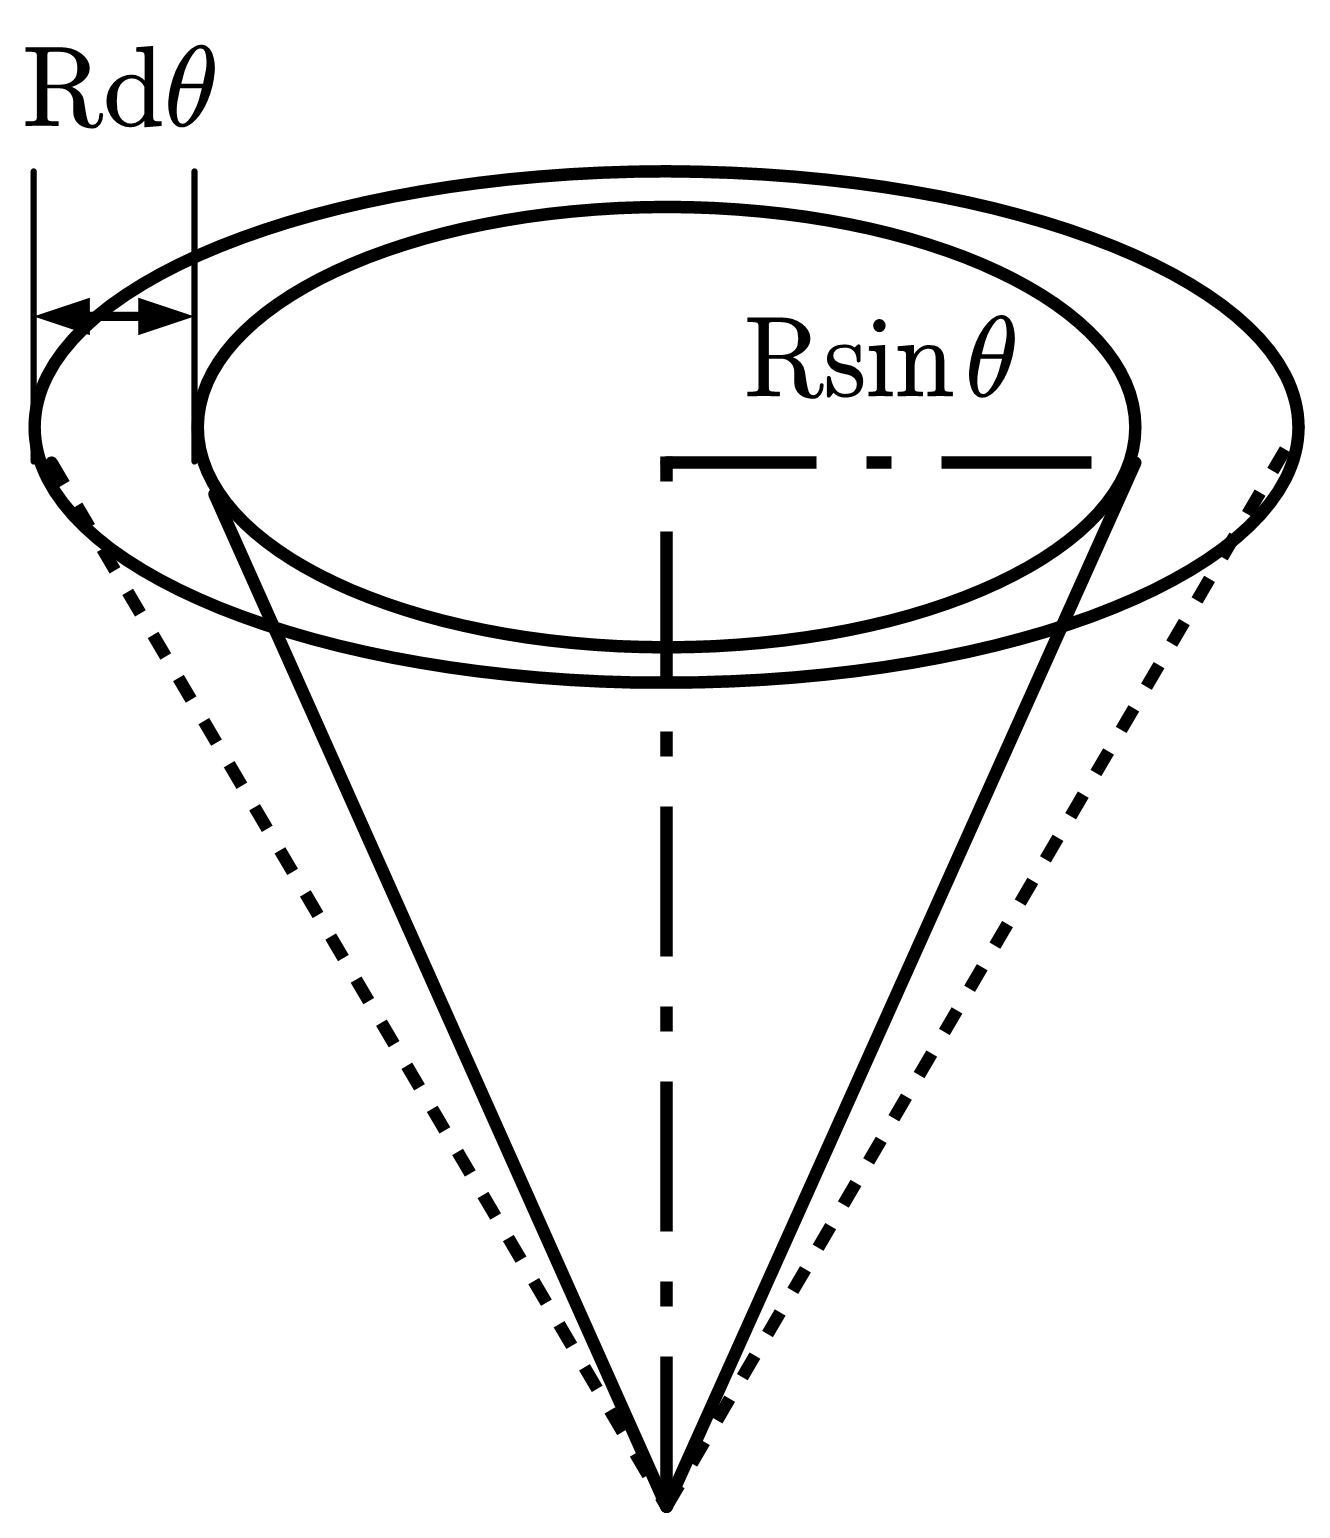
\includegraphics[width=4cm]{figure/NdThetaDist.png}
\end{center}
\subsubsection{常见情形下距离的分布}
\paragraph*{线段}在线段$[0,1]$上随机取2个点,计算距离的分布。

\begin{empheq}{align*}
\Prob(D\leq d)&=\Prob(|x-y|\leq d)\\
&=\Prob(x-d\leq y\leq x+d)
\end{empheq}

对应到正方形中对角梯形的面积,为
$$2\times \frac{\sqrt{2}+\sqrt{2}(1-d)}{2}\frac{d}{\sqrt{2}}=d(2-d)$$

\paragraph*{正方形}在矩形$[0,1]\times[0,1]$上随机取2个点,计算距离的分布。这个就非常复杂了。

